\documentclass[conference]{IEEEtran}

\usepackage[utf8]{inputenc}
\usepackage[T1]{fontenc}
% En Overleaf, opcional para guionado en espanol:
% \usepackage[spanish]{babel}
\usepackage{booktabs}
\usepackage{array}
\usepackage{tabularx}
\usepackage{xcolor}
\usepackage{tikz}
\usetikzlibrary{positioning,arrows.meta}
\usepackage[hidelinks]{hyperref}

\newcolumntype{L}[1]{>{\raggedright\arraybackslash}p{#1}}

\begin{document}

\title{Propuesta de Mejora Arquitect\'onica del\\ Sistema Legacy JWQL}

\author{
\IEEEauthorblockN{Margiory Alvarado Chavez}
\IEEEauthorblockA{Department of Computer Science\\
University of Engineering and Technology\\
Lima, Per\'u\\
margiory.alvarado@utec.edu.pe}
\and
\IEEEauthorblockN{Aaron Coorahua Pe\~na}
\IEEEauthorblockA{Department of Computer Science\\
University of Engineering and Technology\\
Lima, Per\'u\\
ruben.coorahua@utec.edu.pe}
}

\maketitle

\begin{abstract}
JWQL es la aplicaci\'on web con que el STScI monitorea la salud de los instrumentos del telescopio James Webb. Su subsistema de procesamiento es un cuello de botella: la calibraci\'on de im\'agenes, la tarea m\'as costosa, se ejecuta sin paralelismo real y comparte infraestructura con el \textit{dashboard}, de modo que un lote pesado ralentiza el procesamiento y degrada la lectura a la vez. El dato de entrada es adem\'as una rampa de cuatro dimensiones que vuelve la calibraci\'on intensiva en memoria, por lo que el escalado lo limita la RAM por nodo, no la CPU. Proponemos una modernizaci\'on evolutiva (extraer el servicio de calibraci\'on y separar el camino de escritura del de lectura) y un plan de validaci\'on que mide, a recursos fijos, la mejora en latencia y confiabilidad del \textit{dashboard} y el techo de \textit{throughput} seg\'un el tama\~no de imagen.
\end{abstract}

\begin{IEEEkeywords}
arquitectura de software, sistema legacy, Strangler Fig, CQRS, Competing Consumers, Sidecar, escalabilidad
\end{IEEEkeywords}

\section{Introducci\'on}

JWQL es una aplicaci\'on web y \textit{framework} de automatizaci\'on que los equipos de instrumentos del STScI usan para vigilar los cinco instrumentos del telescopio James Webb. Obtiene datos crudos del archivo MAST, los calibra con el \textit{pipeline} cient\'ifico de JWST y ejecuta monitores (corriente de oscuridad, p\'ixeles defectuosos, rayos c\'osmicos, ruido de lectura y telemetr\'ia) cuyos resultados publica en un \textit{dashboard}. Est\'a en producci\'on desde 2017 y su c\'odigo es p\'ublico.\footnote{\url{https://github.com/spacetelescope/jwql}} Este trabajo analiza su arquitectura, define el problema y propone una mejora validable; el dise\~no t\'ecnico y las m\'etricas finales corresponden al siguiente entregable.

\section{Sistema Actual y Problema}

JWQL integra un sistema de archivos de red para los productos calibrados y sin calibrar, una base relacional con los metadatos observacionales, una biblioteca de monitoreo y la aplicaci\'on web de inspecci\'on. Son unos 160 archivos Python y 52 mil l\'ineas de c\'odigo sobre Django, con una cola de tareas as\'incrona en Celery/Redis, PostgreSQL como base de datos y Bokeh para la visualizaci\'on.

El estilo es un monolito en capas con procesamiento as\'incrono parcial (Figura~\ref{fig:asis}): un disparador lanza un monitor, este detecta archivos nuevos, los calibra, guarda resultados y estado en la base, y la web consulta esos datos para armar el \textit{dashboard}.

\begin{figure}[t]
\centering
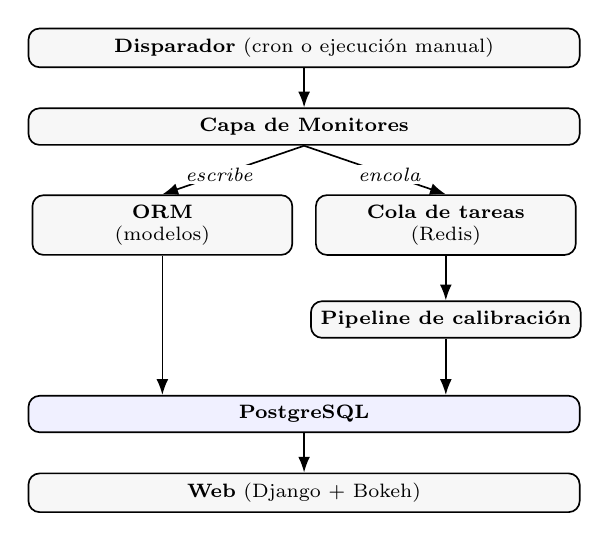
\begin{tikzpicture}[
  font=\scriptsize,
  box/.style={draw, semithick, rounded corners, align=center, inner sep=3.5pt, fill=black!3},
  wide/.style={box, minimum width=7.0cm},
  half/.style={box, minimum width=3.3cm},
  db/.style={box, minimum width=7.0cm, fill=blue!6},
  flow/.style={-{Latex[length=2mm]}, semithick},
  lab/.style={font=\scriptsize\itshape, fill=white, inner sep=1pt}]

\node[wide] (trig) at (0,0) {\textbf{Disparador} (cron o ejecuci\'on manual)};
\node[wide] (mon) at (0,-1.0) {\textbf{Capa de Monitores}};
\node[half] (orm) at (-1.8,-2.25) {\textbf{ORM}\\(modelos)};
\node[half] (cel) at (1.8,-2.25) {\textbf{Cola de tareas}\\(Redis)};
\node[half] (pipe) at (1.8,-3.45) {\textbf{Pipeline de calibraci\'on}};
\node[db] (pg) at (0,-4.65) {\textbf{PostgreSQL}};
\node[wide] (web) at (0,-5.65) {\textbf{Web} (Django + Bokeh)};

\draw[flow] (trig) -- (mon);
\draw[flow] (mon.south) -- (orm.north) node[lab,pos=0.6]{escribe};
\draw[flow] (mon.south) -- (cel.north) node[lab,pos=0.6]{encola};
\draw[flow] (cel) -- (pipe);
\draw[flow] (orm.south) -- (orm.south |- pg.north);
\draw[flow] (pipe.south) -- (pipe.south |- pg.north);
\draw[flow] (pg) -- (web);
\end{tikzpicture}
\caption{Arquitectura actual: monolito en capas con procesamiento as\'incrono parcial.}
\label{fig:asis}
\end{figure}

\subsection{Problema}

El subsistema de procesamiento concentra el problema, por tres causas que se agravan entre s\'i:

\textbf{(P1) Sin paralelismo real.} La cola Celery corre un proceso por worker (\texttt{worker\_concurrency=1}) y reinicia el worker tras cada tarea (\texttt{max\_tasks\_per\_child=1}), y la orquestaci\'on bloquea hasta terminar cada calibraci\'on. La tarea m\'as costosa se ejecuta, en la pr\'actica, en serie.

\textbf{(P2) Acotado por la memoria.} El archivo de entrada (\texttt{uncal}) es una rampa de cuatro dimensiones (columnas $\times$ filas $\times$ grupos $\times$ integraciones) de hasta $\sim$2\,GB (Tabla~\ref{tab:datos}); el ajuste de rampa la carga completa y mantiene varias copias en RAM. Los comentarios de configuraci\'on de JWQL fijan \texttt{worker\_concurrency=1} porque un proceso de \textit{pipeline} ``puede consumir toda la memoria disponible'', y el c\'odigo trata el error \texttt{Cannot allocate memory} como un fallo conocido. El escalado lo limita la RAM por nodo; la huella exacta se mide en el POC sobre una exposici\'on p\'ublica de MAST.

\textbf{(P3) Lectura y escritura acopladas.} Los monitores comparten infraestructura y modelos con la capa web; un lote pesado degrada directamente la latencia del \textit{dashboard}.

A esto se suman problemas de mantenibilidad: m\'odulos con demasiadas responsabilidades (varios sobre 1\,500 l\'ineas, alguno sobre 3\,000) y una persistencia que mezcla dos ORM sobre dos bases. En s\'intesis: cuando llega un lote, el procesamiento es lento \emph{y} el \textit{dashboard} se degrada, y no se puede escalar porque no hay paralelismo, la memoria pone techo y el monolito acopla ambos caminos.

\begin{table}[h]
\centering
\caption{Tama\~no de los productos del \textit{pipeline}.}
\label{tab:datos}
\begin{tabularx}{\columnwidth}{Xl}
\toprule
\textbf{Producto / unidad} & \textbf{Tama\~no aprox.} \\
\midrule
\textit{Frame} de lectura ($2048\times2048$, uint16) & $\sim$8\,MB \\
Exposici\'on \texttt{uncal} t\'ipica (4D) & 40-90\,MB \\
\texttt{uncal} de series temporales (segmentada) & hasta $\sim$2\,GB \\
Producto calibrado \texttt{rate} (2D, float32) & $\sim$17\,MB \\
\bottomrule
\end{tabularx}
\end{table}

\section{Requerimientos}

El trabajo se centra en el procesamiento y la visualizaci\'on de monitores. Las funciones actuales deben preservarse (Tabla~\ref{tab:rf}) y los atributos de calidad a mejorar se listan en la Tabla~\ref{tab:rnf}. Tres restricciones acotan la soluci\'on: la evoluci\'on debe ser incremental porque el sistema est\'a en producci\'on; el escalado debe ser horizontal por el alto consumo de memoria del \textit{pipeline}; y la prueba de concepto debe correrse localmente.

\begin{table}[h]
\centering
\caption{Requerimientos funcionales.}
\label{tab:rf}
\begin{tabularx}{\columnwidth}{lX}
\toprule
\textbf{ID} & \textbf{Requerimiento} \\
\midrule
RF-1 & Detectar archivos nuevos y disparar el monitoreo. \\
RF-2 & Calibrar cada archivo con el \textit{pipeline} de JWST. \\
RF-3 & Calcular las m\'etricas de monitoreo y guardarlas. \\
RF-4 & Registrar el estado de cada corrida. \\
RF-5 & Publicar los resultados en el \textit{dashboard}. \\
RF-6 & Evitar ejecuciones duplicadas o concurrentes. \\
\bottomrule
\end{tabularx}
\end{table}

\begin{table}[h]
\centering
\caption{Requerimientos no funcionales.}
\label{tab:rnf}
\begin{tabularx}{\columnwidth}{lX}
\toprule
\textbf{Atributo} & \textbf{Objetivo} \\
\midrule
Escalabilidad & Procesar varios archivos en paralelo sumando workers. \\
Rendimiento & Reducir el tiempo total de una corrida. \\
Mantenibilidad & Reducir el tama\~no y el acoplamiento de los m\'odulos. \\
Desplegabilidad & Escalar el procesamiento sin afectar la web. \\
Resiliencia & Recuperarse si falla un worker sin perder la corrida. \\
\bottomrule
\end{tabularx}
\end{table}

\section{Usuario Modelo}

El usuario principal es el \textbf{cient\'ifico de instrumento}: necesita detectar tendencias an\'omalas cuanto antes y que el \textit{dashboard} refleje los datos nuevos sin demora; hoy, con un lote grande, el procesamiento tarda horas y la web se vuelve lenta. El usuario secundario es el \textbf{ingeniero que mantiene JWQL}: necesita modificar o agregar monitores y escalar el procesamiento sin afectar otros componentes.

\section{Estado del Arte}

Modernizar un sistema legacy en producci\'on conviene hacerlo de forma evolutiva. El patr\'on \textbf{Strangler Fig} de Fowler~\cite{fowler2004} construye el nuevo sistema alrededor del existente y lo reemplaza poco a poco, sin reescritura total; Newman~\cite{newman2019} aporta t\'acticas para ello, como \textbf{Branch by Abstraction} (aislar un componente tras una interfaz) y \textbf{Parallel Run} (correr ambas implementaciones y comparar). Para una tarea pesada detr\'as de una cola, Richardson~\cite{richardson2018} propone \textbf{Competing Consumers}: varios workers compiten por la misma cola y el rendimiento crece con su n\'umero. El patr\'on \textbf{CQRS}~\cite{youngcqrs} separa el camino de escritura del de lectura para escalarlos por separado, lo que importa cuando hay contenci\'on de recursos entre ambos.

Li, Ma y Lu~\cite{lima2020} aplicaron esta combinaci\'on en el sistema Green Button: extrajeron con Strangler Fig y CQRS el servicio que era cuello de botella y midieron el impacto a recursos fijos. Su resultado es la clave metodol\'ogica que adoptamos: el efecto m\'as importante no fue sobre el servicio migrado, sino sobre el resto del sistema, ya que los m\'odulos no migrados mejoraron su tiempo de respuesta al liberarse los recursos que consum\'ia el componente pesado. La arquitectura original de JWQL est\'a documentada por Bourque et al.~\cite{bourque2020}.

\section{Propuesta}

El foco son P1, P2 y P3 (el cuello de botella de procesamiento). La propuesta es una \textbf{modernizaci\'on evolutiva en un solo corte}: extraer el servicio de calibraci\'on detr\'as de una interfaz, separar el camino de escritura del de lectura y mantener el camino actual operativo durante la transici\'on. No es una migraci\'on completa a microservicios ni una reescritura. La implementaci\'on se desarrollar\'a en \url{https://github.com/AaronCoorahua/jwql-arch-evolution}.

La Tabla~\ref{tab:patrones} resume los patrones. El \textbf{benchmark prueba} el efecto de Competing Consumers (escalado) y CQRS (separaci\'on lectura/escritura); Strangler Fig y Branch by Abstraction son el \emph{m\'etodo} de extracci\'on incremental; el Sidecar provee la observabilidad.

\begin{table}[h]
\centering
\caption{Patrones de la propuesta.}
\label{tab:patrones}
\begin{tabularx}{\columnwidth}{XL{3.4cm}}
\toprule
\textbf{Objetivo} & \textbf{Patr\'on} \\
\midrule
Paralelizar la calibraci\'on & Competing Consumers \\
Separar lectura de escritura & CQRS + r\'eplicas de lectura \\
Aislar el \textit{pipeline} & Branch by Abstraction \\
Migrar sin detener el sistema & Strangler Fig + Parallel Run \\
Observabilidad sin tocar el core & Sidecar \\
\bottomrule
\end{tabularx}
\end{table}

\subsection{Hip\'otesis}

A recursos totales fijos, (i)~separar escritura de lectura reduce la latencia y la tasa de error del \textit{dashboard} mientras corre un lote (efecto de mayor impacto que solo a\~nadir workers), y (ii)~el \textit{throughput} de procesamiento se satura por memoria antes que por CPU, con un techo que depende del tama\~no de imagen.

\subsection{Experimento}

El cuello de botella es la calibraci\'on (P1, P2). Se mide su rendimiento antes y despu\'es de extraerla, a igualdad de recursos (CPU y RAM fijos en contenedores Docker), con el dise\~no de Li, Ma y Lu~\cite{lima2020}: se eligen dos componentes bajo prueba (AUT) y se compara cada uno antes y despu\'es de la mejora.

\begin{itemize}
\item \textbf{AUT-1, procesamiento (escritura):} la calibraci\'on \texttt{calwebb\_detector1} que dispara el dark monitor v\'ia \texttt{shared\_tasks.run\_pipeline}. Es el componente que se extrae.
\item \textbf{AUT-2, dashboard (lectura):} la vista \texttt{dark\_monitor(inst)} de \texttt{monitor\_views.py}, que arma las pesta\~nas Bokeh leyendo de la base \texttt{monitors} (endpoint \texttt{GET /<inst>/dark\_monitor/}). Es el componente no migrado que comparte recursos con el procesamiento.
\end{itemize}

La carga es de 200 hilos por 5 repeticiones por AUT, como en~\cite{lima2020}, y se repite con dos tama\~nos de exposici\'on (\texttt{rate} peque\~no y \texttt{uncal} grande) para observar el techo de memoria. Se ejecuta el stack real de JWQL (web, Celery, Redis y PostgreSQL) en contenedores; el \textit{pipeline} se sustituye por una carga sint\'etica calibrada contra una corrida real sobre datos p\'ublicos de MAST/CRDS, para fijar el perfil de CPU y memoria. CPU y RAM se recolectan a nivel de nodo (en producci\'on, v\'ia un \textit{sidecar} por servicio). Para cada AUT se reportan las m\'etricas de la Tabla~\ref{tab:metricas} antes y despu\'es.

\begin{table}[h]
\centering
\caption{M\'etricas por AUT, antes y despu\'es de extraer la calibraci\'on. Carga: 200 hilos $\times$ 5.}
\label{tab:metricas}
\begin{tabularx}{\columnwidth}{Xl}
\toprule
\textbf{M\'etrica} & \textbf{Criterio de mejora} \\
\midrule
Tiempo de prueba (s) & menor o igual \\
Respuesta media (ms) & menor en la vista \texttt{dark\_monitor} (lectura) \\
Error (\%) & tiende a 0 \\
\textit{Throughput} (req/s) & mayor \\
Tama\~no medio de respuesta (B) & igual (control de carga) \\
Pico de RAM por tarea (GB) & caracteriza el techo de escalado \\
\texttt{Cannot allocate memory} (conteo) & tiende a 0 \\
\bottomrule
\end{tabularx}
\end{table}

\subsection{Resultado esperado}

Como en Green Button, se espera que el componente no migrado, la vista \texttt{dark\_monitor}, sea el que m\'as mejore: su respuesta media y su tasa de error bajo carga deben caer al dejar de competir por los recursos de la calibraci\'on. En el procesamiento (\texttt{calwebb\_detector1}) se espera mayor \textit{throughput} al sumar workers y la desaparici\'on de los errores de memoria. Las cifras se obtienen en el siguiente entregable.

\begin{thebibliography}{9}
\bibitem{bourque2020} M. Bourque et al., ``The James Webb Space Telescope Quicklook Application (JWQL),'' \textit{ASP Conf. Ser.}, vol. 527, p. 539, 2020. Software: Zenodo, doi: 10.5281/zenodo.3698708.
\bibitem{fowler2004} M. Fowler, ``StranglerFigApplication,'' martinfowler.com, 2004.
\bibitem{newman2019} S. Newman, \textit{Monolith to Microservices}. O'Reilly Media, 2019.
\bibitem{richardson2018} C. Richardson, \textit{Microservices Patterns}. Manning Publications, 2018.
\bibitem{youngcqrs} M. Fowler, ``CQRS,'' martinfowler.com.
\bibitem{lima2020} C.-Y. Li, S.-P. Ma, and T.-W. Lu, ``Microservice Migration Using Strangler Fig Pattern: A Case Study on the Green Button System,'' in \textit{2020 Int. Computer Symposium (ICS)}, pp. 519--524, IEEE.
\end{thebibliography}

\end{document}
